% !TEX root = ../main.tex
\subsubsection{Efficiency Study}
\label{14.14::efficiency_study}
% --+ Integrated. +-------------------------------------------------------------
    With all these effects accounted for, we can proceed to study the efficiency in detail.
    First, if we define FMT efficiency as the percentage of DC tracks that get accepted by FMT, we get the results in Table \ref{tab::14.14::fmt_efficiency_study} for runs 12933 (Summer 2020) and 12016 (Spring 2020), as well as the simulation described in Section \ref{13.40::acceptance_correction}.

    \begin{table}[b]
        \begin{center}
            \begin{tabularx}{0.86\textwidth}{Xlcrrcrr}
                \toprule
                & & & \multicolumn{2}{c}{\textbf{Run 12933}} & & \multicolumn{2}{c}{\textbf{Run 12016}} \\
                                    &          & & \multicolumn{1}{c}{raw} & \multicolumn{1}{c}{w/ cut} & & \multicolumn{1}{c}{raw} & \multicolumn{1}{c}{w/ cut} \\
                \midrule \midrule
                \textbf{$e^-$}      & 2 layers & & $25.1 \pm 1.5$ & $37.5 \pm 0.7$ & & $32.7 \pm 2.5$ & $53.7 \pm 0.8$ \\
                                    & 3 layers & & $ 5.6 \pm 2.7$ & $ 8.5 \pm 1.7$ & & $ 9.9 \pm 6.3$ & $16.4 \pm 3.6$ \\
                \midrule
                \textbf{$e^-\pi^+$} & 2 layers & & $ 6.5 \pm 0.2$ & $13.7 \pm 0.9$ & & $11.1 \pm 0.2$ & $28.0 \pm 1.3$ \\
                                    & 3 layers & & $ 0.3 \pm 0.1$ & $ 0.7 \pm 0.4$ & & $ 1.0 \pm 0.1$ & $ 2.7 \pm 1.4$ \\
                \midrule
                \textbf{$e^-\pi^-$} & 2 layers & & $ 5.6 \pm 0.0$ & $14.2 \pm 1.0$ & & $ 8.9 \pm 0.4$ & $29.5 \pm 1.4$ \\
                                    & 3 layers & & $ 0.3 \pm 0.0$ & $ 0.7 \pm 0.5$ & & $ 0.9 \pm 0.3$ & $ 2.9 \pm 1.6$ \\
                \bottomrule
            \end{tabularx}
        \end{center}
        \caption[FMT efficiency study results]
        {Results of the FMT efficiency study performed in $\%$.}
        \label{tab::14.14::fmt_efficiency_study}
    \end{table}

    % --+ Error estimation +----------------------------------------------------
    To estimate the efficiency of one FMT layer and the associated errors for the two types of tracks, we define $P(L_n)$ as the probability of layer $n$ detecting a particle, with $1 \leq n \leq 3$.
    Assuming that all layers have the same efficiency, denoted as $E_1$,
    \begin{equation*}
        P(L_1) = P(L_2) = P(L_3) = E_1,
    \end{equation*}
    the efficiency $E_3$ for 3-layer tracks can be obtained using the probabilities $P(L_n)$ as follows
    \begin{align}
        E_3 &= P(L_1)P(L_2)P(L_3)
        \nonumber \\
        E_3 &= E_{1(3)}^3,
        \label{eq::14.14::efficiency3}
    \end{align}
    where $E_{1(3)}$ is the 1-layer efficiency estimated from 3-layer tracks.

    For 2-layer tracks, the efficiency $E_2$ can be obtained as
    \begin{align}
        E_2 &= P(L_1)P(L_2)\left(1 - P(L_3)\right)                \nonumber \\
             &\hspace{24pt} + P(L_2)P(L_3)\left(1 - P(L_1)\right) \nonumber \\
             &\hspace{24pt} + P(L_3)P(L_1)\left(1 - P(L_2)\right) \nonumber \\
             &\hspace{24pt} + P(L_1)P(L_2)P(L_3)                  \nonumber \\
        E_2 &= 3E_{1(2)}^2\left(1 - E_{1(2)}\right) + E_{1(3)}^3
            \nonumber \\
        E_2 &= 3E_{1(2)}^2 \cdot \left( 1 - E_{1(2)} \right) + E_3,
        \label{eq::14.14::efficiency2}
    \end{align}
    where $E_{1(2)}$ is the 1-layer efficiency estimated from 2-layer tracks.

    From \eqref{eq::14.14::efficiency3}, we can estimate $E_{1(3)}$ as
    \begin{equation}
        E_{1(3)} = \sqrt[3]{E_3}.
        \label{eq::14.14::efficiency1(3)}
    \end{equation}
    In contrast, $E_{1(2)}$ cannot be obtained explicitly from \eqref{eq::14.14::efficiency2}, but it can be estimated numerically.

    Using equations \eqref{eq::14.14::efficiency2} and \eqref{eq::14.14::efficiency1(3)}, we can estimate the weighted average efficiency $\xoverline{E_1}$ as
    \begin{equation*}
        \xoverline{E_1} = \frac{4E_{1(2)} + E_{1(3)}}{5},
    \end{equation*}
    where the weights are assigned based on the number of ways 2 and 3-layer tracks can be obtained, 4 and 1, respectively.

    From $\xoverline{E_1}$, we can estimate the errors on $E_{1(2)}$ and $E_{1(3)}$ as
    \begin{align*}
        \delta(E_{1(2)}) = |\xoverline{E_1} - E_{1(2)}|, \\
        \delta(E_{1(3)}) = |\xoverline{E_1} - E_{1(3)}|.
    \end{align*}

    To propagate these errors to the efficiencies $E_2$ and $E_3$, we use the variance formula
    \begin{equation*}
        \delta\left(f(x)\right) = \frac{\partial f(x)}{\partial x} \cdot \delta(x),
    \end{equation*}
    where $\delta(E_2)$, obtained from equation \eqref{eq::14.14::efficiency2}, is
    \begin{align*}
        \delta(E_2) &= \frac{\partial}{\partial E_{1(2)}} \left( 3E_{1(2)}^2 - 3E_{1(2)}^3 + E_{1(3)}^3 \right)
            \cdot \delta \left( E_{1(2)} \right) \\
        \delta(E_2) &= \left( 6E_{1(2)} - 9E_{1(2)}^2 \right) \cdot \delta \left( E_{1(2)} \right)
    \end{align*}
    and $\delta(E_3)$, obtained from equation \eqref{eq::14.14::efficiency3}, is
    \begin{align*}
        \delta(E_3) &= \frac{\partial}{\partial E_{1(3)}} \left( E_{1(3)}^3 \right) \cdot \delta \left( E_{1(3)} \right) \\
        \delta(E_3) &= 3E_{1(3)}^2 \cdot \delta \left( E_{1(3)} \right).
    \end{align*}

    A Python procedure was written to calculate $E_2$ and $E_3$ from each measurement shown in Table \ref{tab::14.14::fmt_efficiency_study}.
    The corresponding errors were obtained this way, and are included in the table.

    % --+ Conclusions drawn from table +----------------------------------------
    The table illustrates the positive impact of switching to Spring 2020 data and applying the geometry cut.
    The switch results in a $30.1\%$ increase in detected trigger electrons, as well as a $70.8\%$ increase for positive pions and a $58.9\%$ increase for negative pions.
    Furthermore, by applying the geometry cut based on $v_z$ and $\theta$, an additional $64.2\%$ increase in trigger electrons is achieved, resulting in a total increase of $113.9\%$.
    The pion yield experiences a substantial enhancement, with positive pions increasing by $150.2\%$ and negative pions increasing by $231.5\%$, resulting in a total increase of $330.8\%$ and $426.8\%$, respectively.

% --+ Separated. +--------------------------------------------------------------
    Next, we need to ensure that we are not introducing a systematic error by applying these corrections.
    To achieve this, we must investigate the effect of the geometry cut on different detected variables for electrons ($e^-$), positive pions ($e^-\pi^+$), and negative pions ($e^-\pi^-$).
    Based on the definition of the cut, we anticipate a strong correlation between efficiency and $v_z$ and $\theta$, and at most a weak correlation with $\phi$ and $p$.

    \begin{figure}
        % vz.
        \begin{subfigure}[b]{\textwidth}
            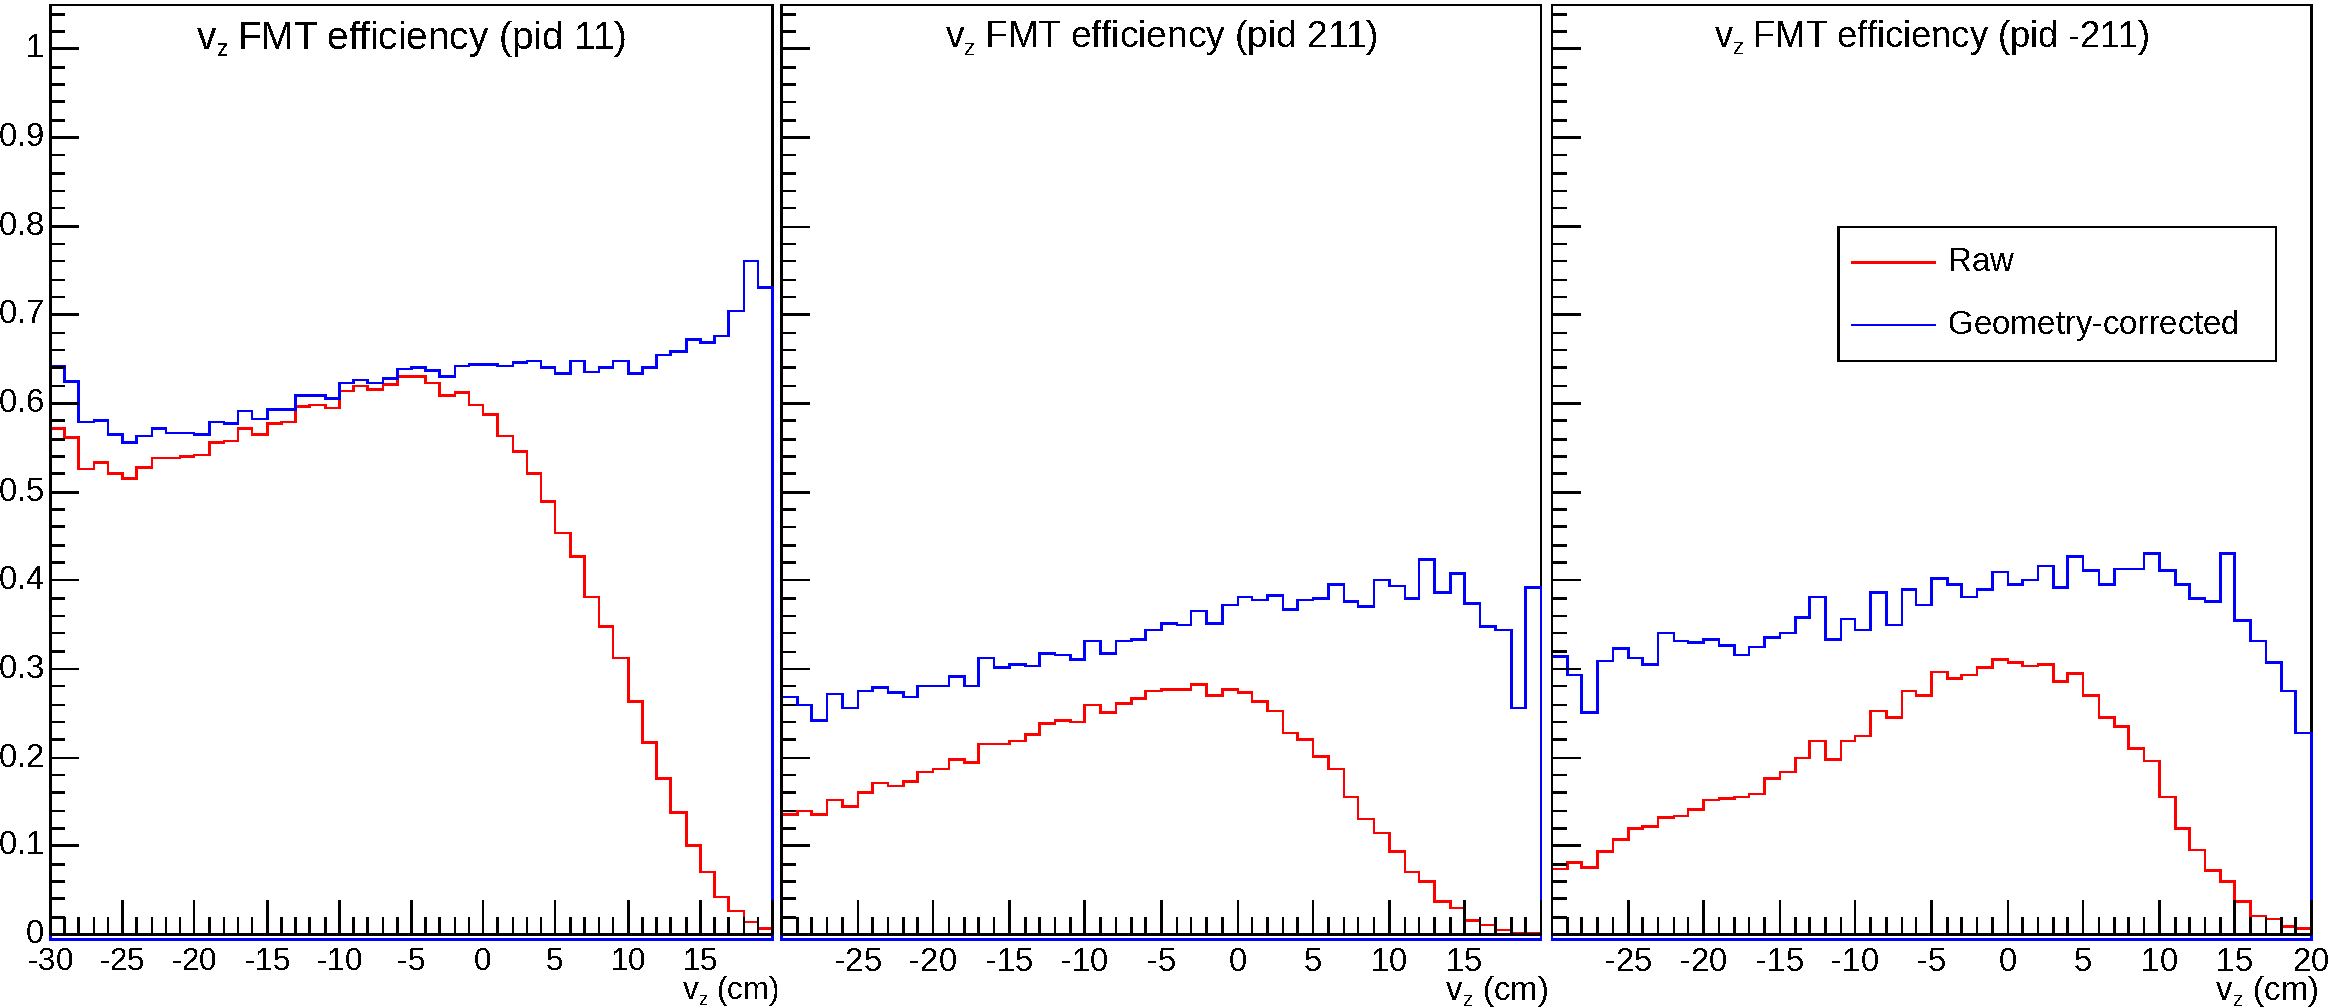
\includegraphics[width=\textwidth]{14vz_efficiency.pdf}
            \caption{$v_z$ FMT efficiency}
            \label{fig::14.14::fmt_efficiency_vz}
        \end{subfigure}
        % theta.
        \begin{subfigure}[b]{\textwidth}
            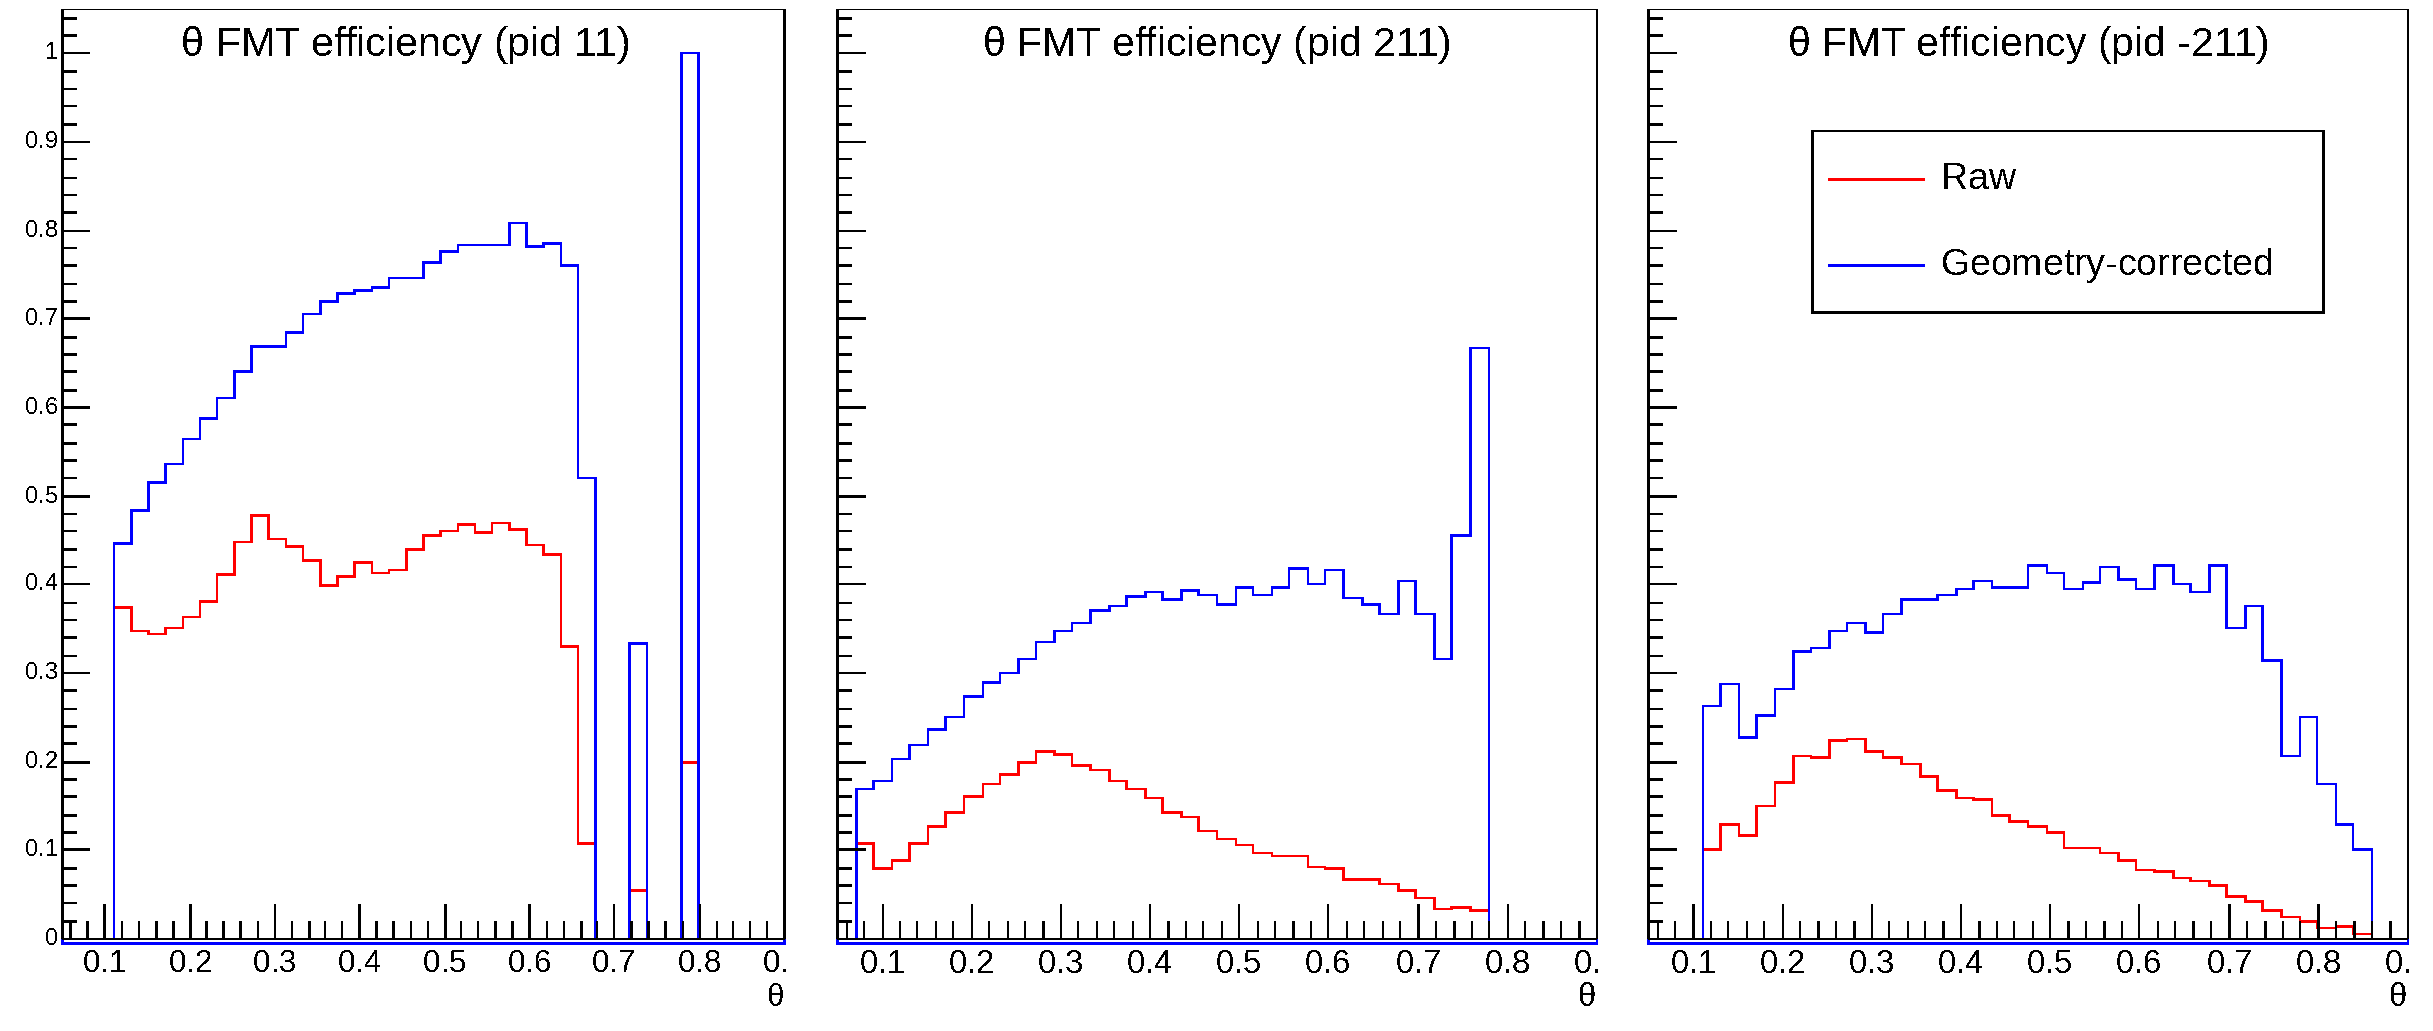
\includegraphics[width=\textwidth]{14theta_efficiency.pdf}
            \caption{$\theta$ FMT efficiency.}
            \label{fig::14.14::fmt_efficiency_theta}
        \end{subfigure}
        % p.
        \begin{subfigure}[b]{\textwidth}
            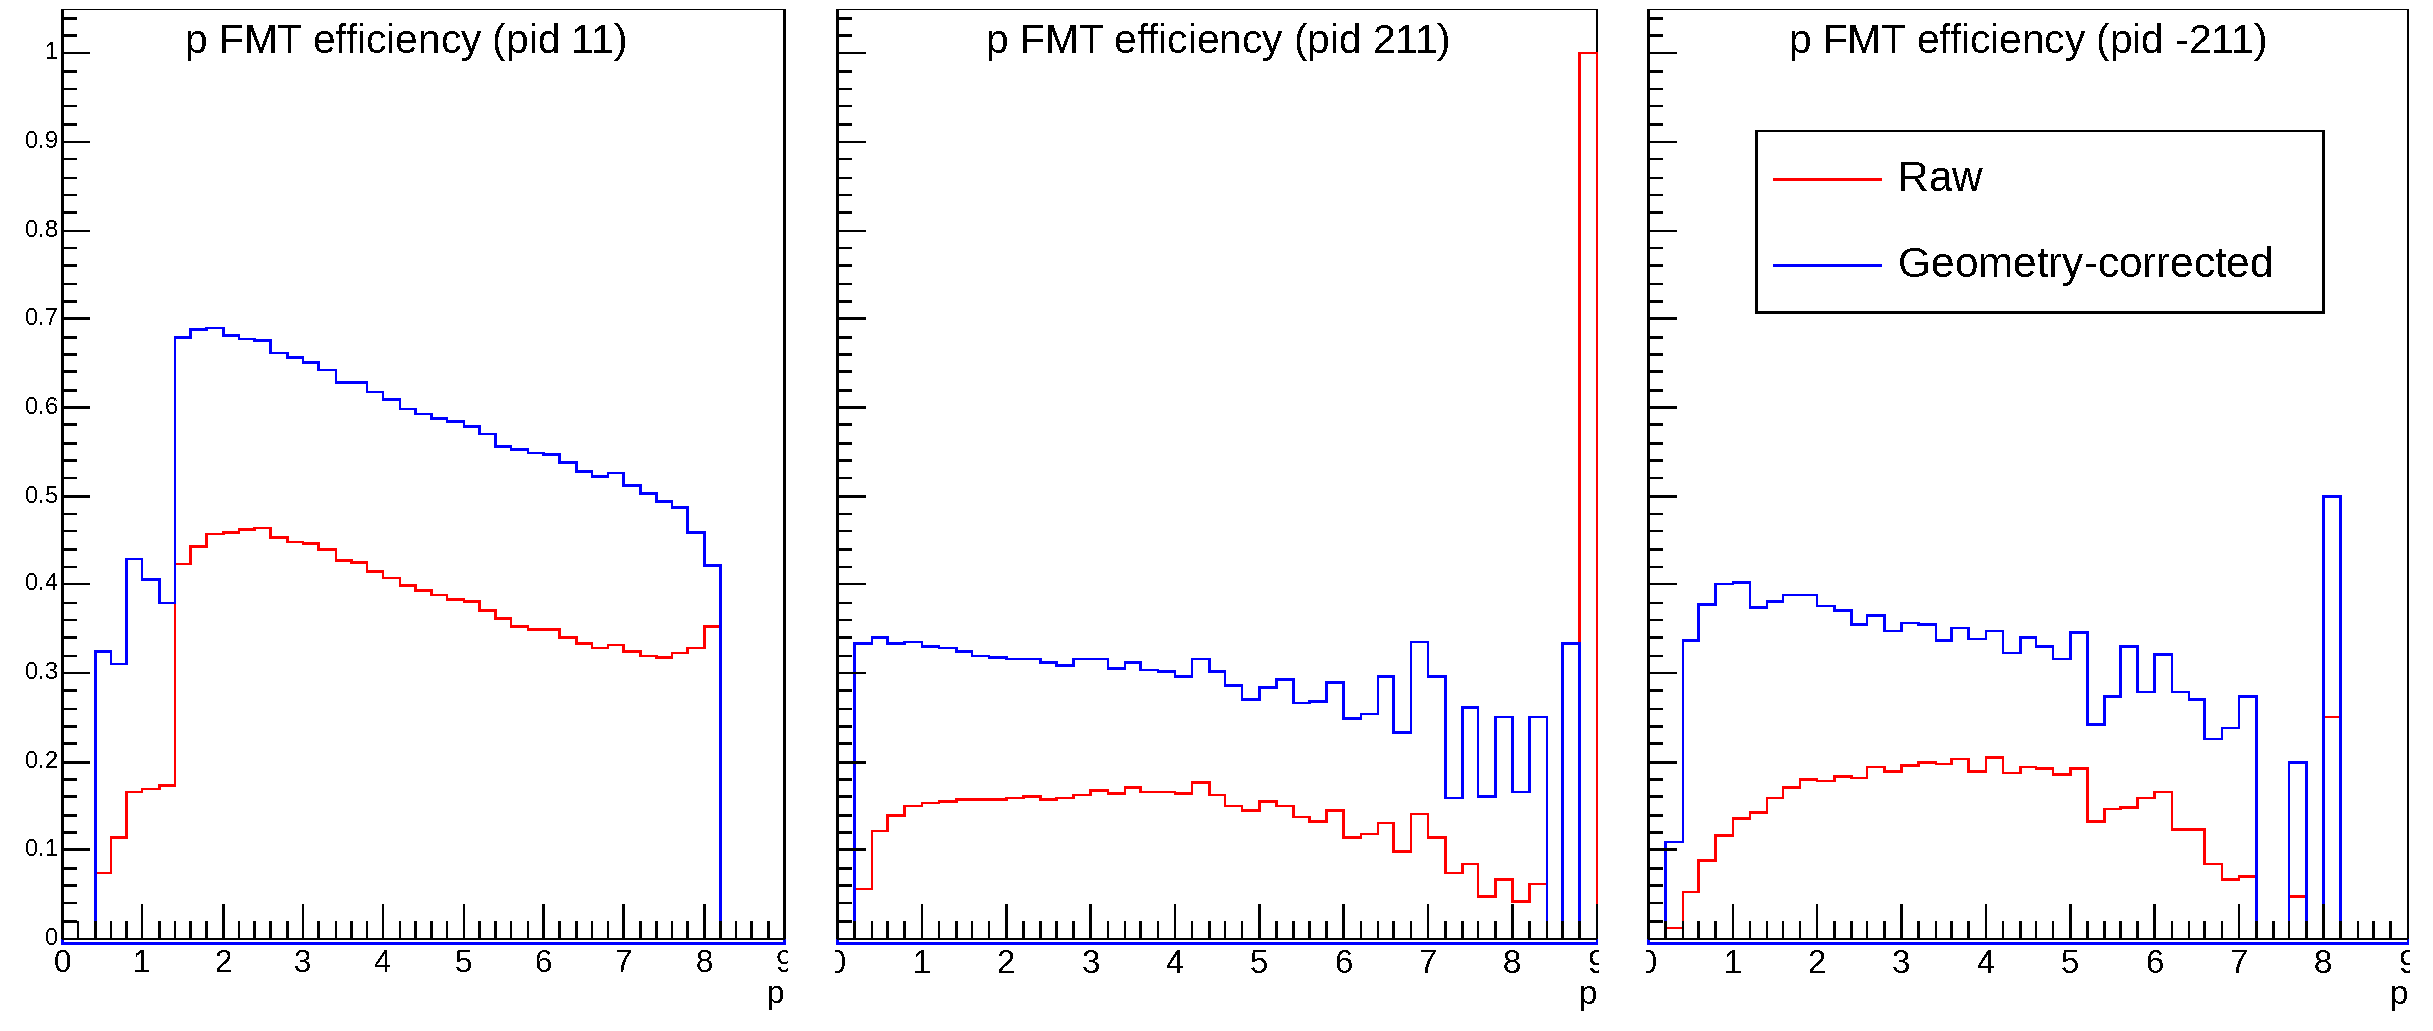
\includegraphics[width=\textwidth]{14p_efficiency.pdf}
            \caption{$p$ FMT efficiency.}
            \label{fig::14.14::fmt_efficiency_p}
        \end{subfigure}

        \caption[$v_z$, $\theta$, and $p$ FMT efficiencies for $e^-$, $e^-\pi^+$, and $e^-\pi^-$]
        {$v_z$, $\theta$, and $p$ FMT efficiencies for $e^-$, $e^-\pi^+$, and $e^-\pi^-$.
        FMT efficiency is defined as the percentage of DC tracks that are detected by 2 FMT layers.
        Run 12016.}
        \floatfoot{Source: Own elaboration, using the \href{https://github.com/bleaktwig/clas12-rge-analysis}{clas12-rge-analysis} software.}
        \label{fig::14.14::fmt_efficiencies}
    \end{figure}

    \begin{figure}
        % phi efficiency.
        \begin{subfigure}[b]{\textwidth}
            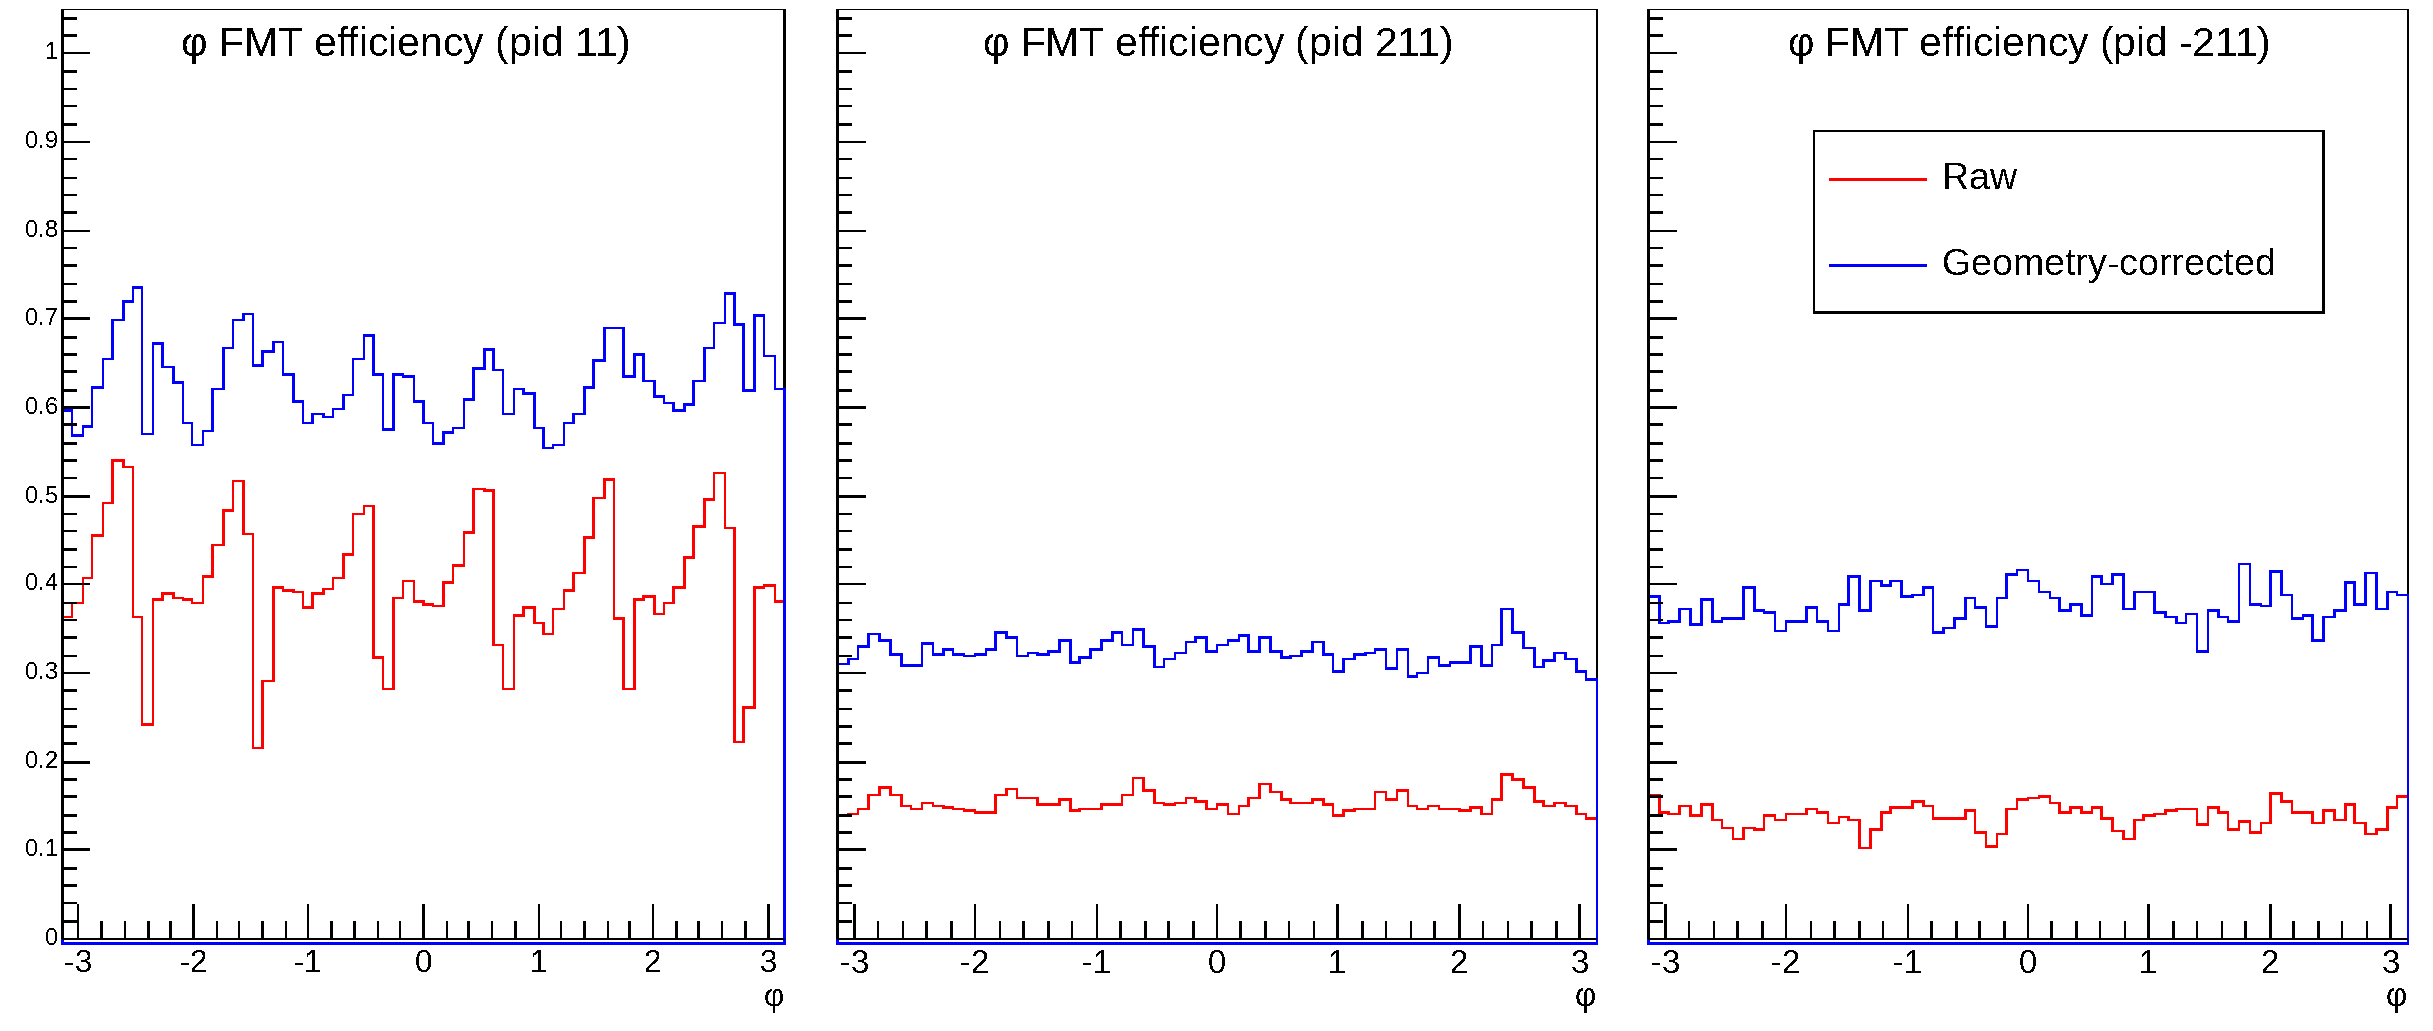
\includegraphics[width=\textwidth]{14phi_efficiency.pdf}
            \caption{$\phi$ FMT efficiency for $e^-$, $e^-\pi^+$, and $e^-\pi^-$.
            FMT efficiency is defined as the percentage of DC tracks that are detected by 2 FMT layers.}
            \label{fig::14.14::fmt_efficiency_phi}
        \end{subfigure}
        % geometry cut effect.
        \begin{subfigure}[b]{\textwidth}
            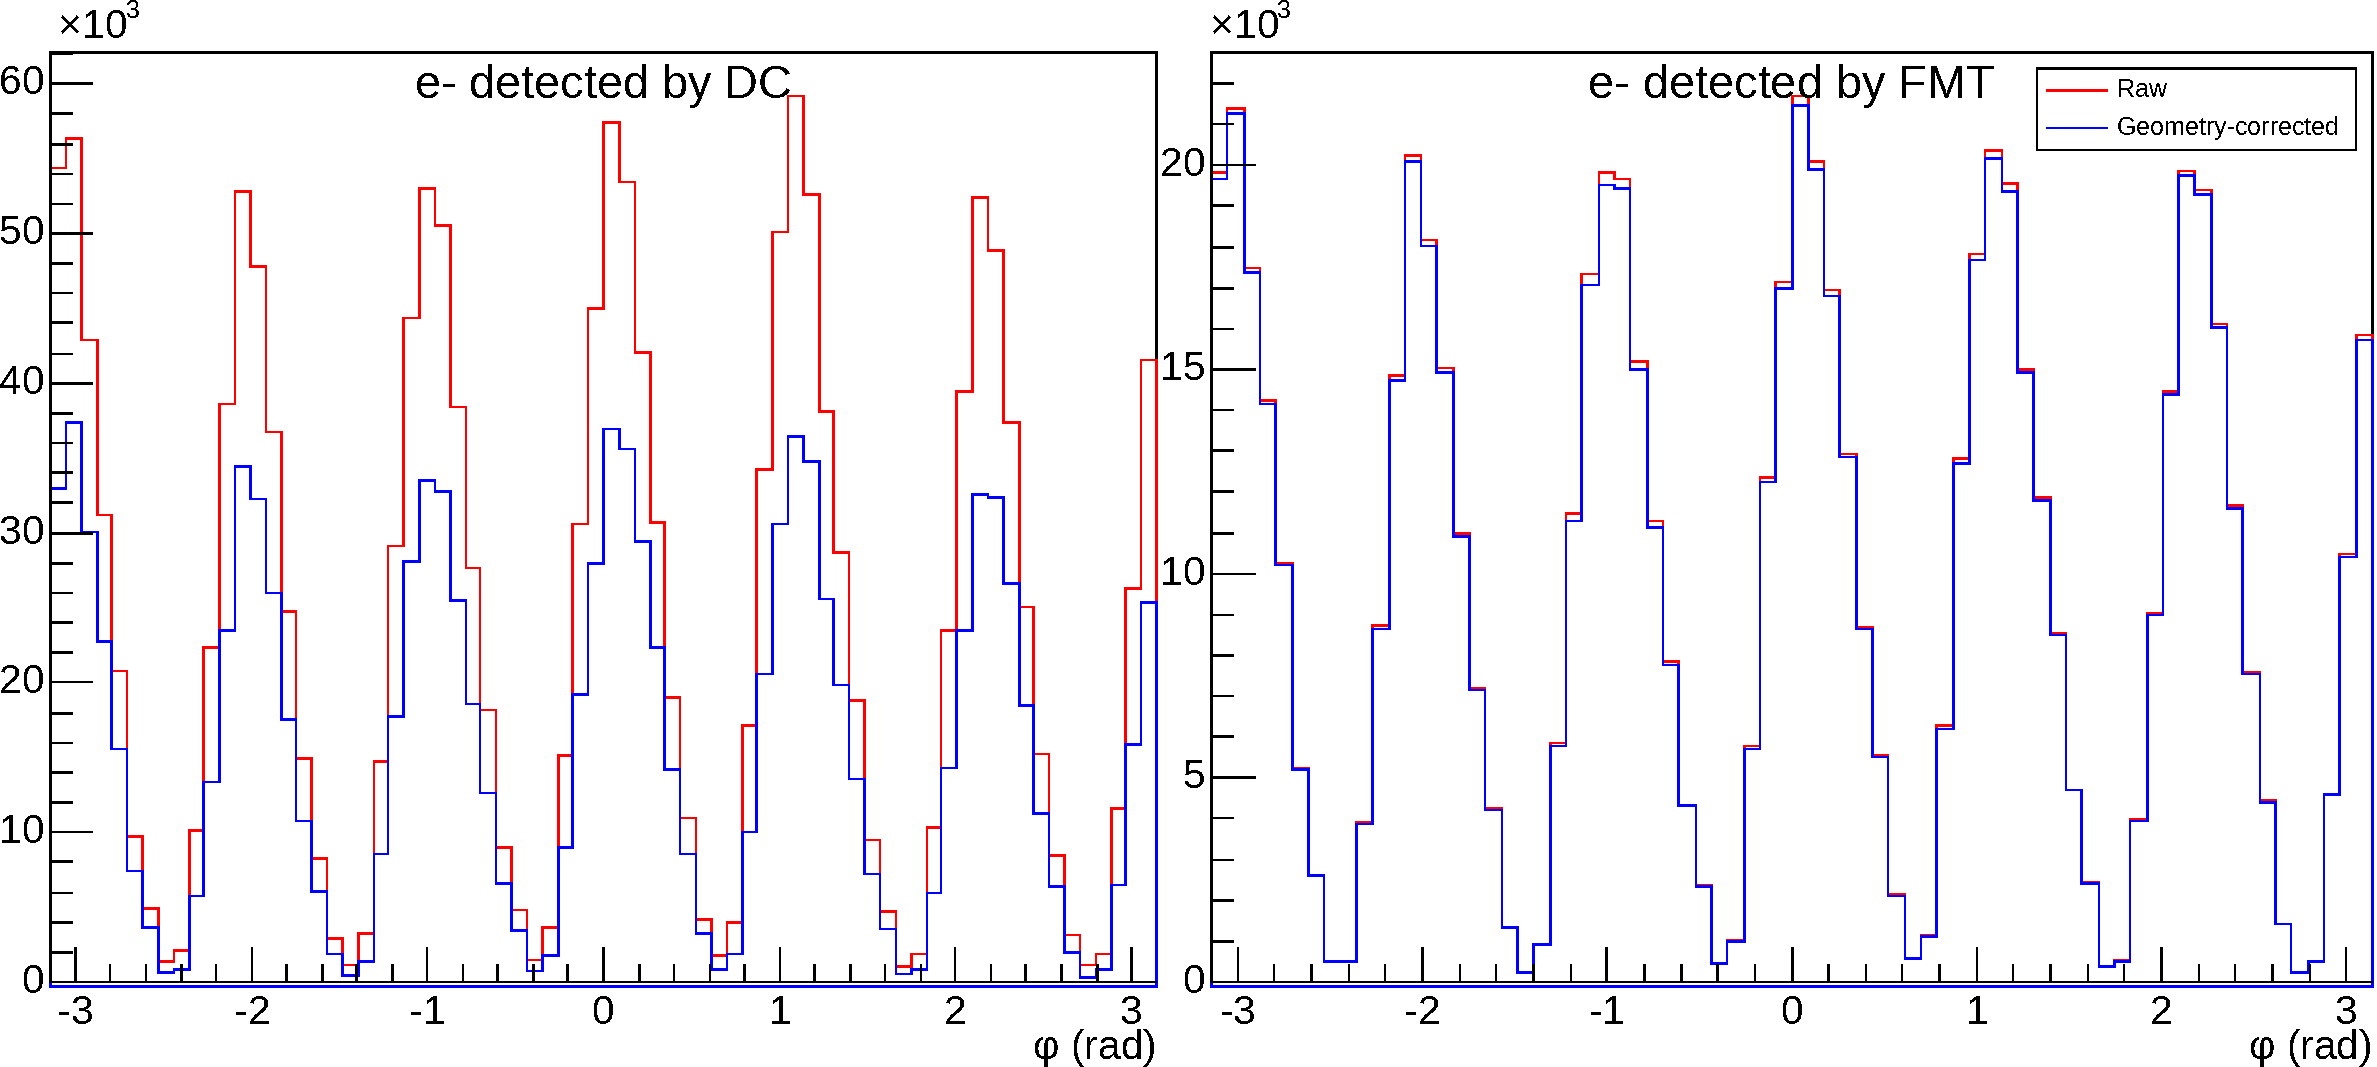
\includegraphics[width=\textwidth]{14phi_geomcut.pdf}
            \caption{Number of electrons detected in terms of $\phi$ for DC and FMT.}
            \label{fig::14.14::phi_geomcut}
        \end{subfigure}

        \caption[$\phi$ efficiency and geometry cut study]
        {$\phi$ FMT efficiency and number of $e^-$ detected for DC and FMT.
        Run 12016.}
        \floatfoot{Source: Own elaboration, using the \href{https://github.com/bleaktwig/clas12-rge-analysis}{clas12-rge-analysis} software.}
        \label{fig::14.14::phi_study}
    \end{figure}

    Our prediction is validated by Figures \ref{fig::14.14::fmt_efficiency_vz} and \ref{fig::14.14::fmt_efficiency_theta}.
    The efficiency displays a pronounced dependence on both $v_z$ and $\theta$ for all three particles under study.
    It is worth noting that the dependence is more pronounced for electrons compared to pions.
    This outcome aligns with expectations, as the only accepted pions are those detected in events where an electron is also detected.
    Thus, the ``final'' pion efficiency incorporates the combined detector efficiencies for electrons and pions.

    Next, Figure \ref{fig::14.14::fmt_efficiency_p} confirms our expectation that there is no strong correlation between efficiency and momentum.

    Last, we examine the $\phi$ efficiency, as depicted in Figure \ref{fig::14.14::fmt_efficiency_phi}.
    Our prediction holds true for both positive and negative pions, as the efficiency demonstrates no dependence on the value of $\phi$.
    However, in the case of electrons, upon initial inspection, the sharp valleys appear less prominent after applying the geometry cut.

    Nevertheless, this is merely a visual effect.
    When we tally the number of electrons detected by the DC and FMT, the valleys become more pronounced in the DC, while they remain the same in the FMT.
    Consequently, the increase in FMT efficiency becomes more pronounced in these valleys, as demonstrated in Figure \ref{fig::14.14::phi_geomcut}.

    As can be seen in Table \ref{tab::14.14::fmt_efficiency_study} and Figures \ref{fig::14.14::fmt_efficiencies} and \ref{fig::14.14::phi_study}, the pion efficiency for 3-layer tracks does not exceed $3\%$.
    Consequently, it is not practical to work exclusively with FMT tracks that traverse all three FMT layers in this study.
    For the remainder of the document, 2 and 3-layer tracks will be considered together, and will be collectively referred to as FMT tracks.
